%
% CSE Electronic Homework Template
% Last modified 8/20/2019 by Jeremy Buhler

\documentclass[11pt]{article}
\usepackage[left=0.7in,right=0.7in,top=1in,bottom=0.7in]{geometry}
\usepackage{fancyhdr} % for header
\usepackage{graphicx} % for figures
\usepackage{amsmath}  % for extended math markup
\usepackage{amssymb}
\usepackage{amsthm}
\usepackage{tikz}
\usepackage[noend]{algpseudocode} % for pseudocode
\usepackage[plain]{algorithm} % float environment for algorithms

\usetikzlibrary{graphs.standard}

%%%%%%%%%%%%%%%%%%%%%%%%%%%%%%%%%%%%%%%%%%%%%%%%%%%%%%%%%%%%%%%%%%%%%%
% STUDENT: modify the following fields to reflect your the current
% homework number.  Do NOT include a name or ID or other personally
% identifying info, as we will use anonymized grading in GradeScope.

\newcommand{\HomeworkNumber}{5}

%%%%%%%%%%%%%%%%%%%%%%%%%%%%%%%%%%%%%%%%%%%%%%%%%%%%%%%%%%%%%%%%%%%%%%%%
% You can pretty much leave the stuff up to the next line of %%'s alone.

% create header and footer for every page
\pagestyle{fancy}
\fancyhf{}
\rhead{\textbf{Hwk \HomeworkNumber{}}}
\cfoot{\thepage}

% preferred pseudocode style
\algrenewcommand{\algorithmicprocedure}{}
\algrenewcommand{\algorithmicthen}{}

% ``do { ... } while (cond)''
\algdef{SE}[DOWHILE]{Do}{doWhile}{\algorithmicdo}[1]{\algorithmicwhile\ #1}%

% ``for (x in y ... z)''
\newcommand{\ForRange}[3]{\For{#1 \textbf{in} #2 \ \ldots \ #3}}

% these are common math formatting commands that aren't defined by default
\newcommand{\union}{\cup}
\newcommand{\isect}{\cap}
\newcommand{\ceil}[1]{\ensuremath \left\lceil #1 \right\rceil}
\newcommand{\floor}[1]{\ensuremath \left\lfloor #1 \right\rfloor}

\newtheorem{lem}{Lemma}
\newtheorem{thm}{Theorem}

%%%%%%%%%%%%%%%%%%%%%%%%%%%%%%%%%%%%%%%%%%%%%%%%%%%%%%%%%%%%%%%%%%%%%%

\begin{document}

\section{}
\subsection*{a.}
\begin{lem} 
    \label{thm:min-same}  
    At least $\frac{n}{k}$ tellers share a code.

\end{lem}
\begin{proof}
    Suppose no code was shared by more than $\frac{n}{k} - 1$ tellers. Since there are $k$ codes, this would imply that there are at most $(\frac{n}{k} - 1)k = n - k$ tellers, contradiction the assumption that there are $n$ tellers. Therefore the assumption must be false, and a code exists which is shared by at least $\frac{n}{k}$ tellers.
\end{proof}

Suppose $m$ tellers share a code. These tellers must not be assigned to work at the same time, so within a valid shift graph, there must not be an edge between any of the $m$ tellers. Therefore a group of $m$ tellers who share the same vault code forms an independent set of size $m$ within the shift graph. By Lemma \ref{thm:min-same}, for $n$ tellers and $k$ codes, at least $\frac{n}{k}$ tellers will share a single code, so in a valid graph, there must be an independent set of size $\frac{n}{k}$.

\subsection*{b.}
The obvious reduction from ISET would be to identify the maximum independent set within the graph, assign the set a single code, remove the set from the graph, and repeat until all vertices have been removed from the graph. 
 However, this approach fails for certain graphs, where it is more efficient to eliminate a well-connected vertex earlier in the process. Consider the graph 
 \begin{figure}[H]
    \centering
    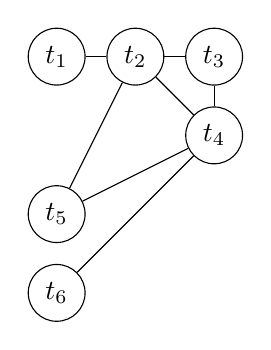
\begin{tikzpicture}
        \graph[nodes={circle, draw}] {
            "$t_1$" -- "$t_2$" -- {"$t_3$", "$t_4$"};
            "$t_4$" -- {"$t_5$", "$t_6$"};
            "$t_3$" -- "$t_4$";
            "$t_2$" -- "$t_5$";
        };
    \end{tikzpicture}
 \end{figure}

 The maximum independent set is of size $3$ and consists of tellers $t_1, t_5$ and $t_6$ or $t_1, t_3, $ and $t_6$. After eliminating each of these, the resultant graphs are 
 \begin{figure}[H]
    \centering
    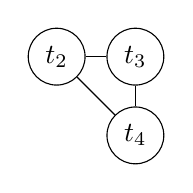
\begin{tikzpicture}
        \graph[nodes={circle, draw}] {
            "$t_2$" -- {"$t_3$", "$t_4$"};
            "$t_3$" -- "$t_4$";
        };
    \end{tikzpicture}, and
    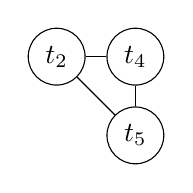
\begin{tikzpicture}
        \graph[nodes={circle, draw}] {
            "$t_2$" -- {"$t_4$", "$t_5$"};
            "$t_4$" -- "$t_5$";
        };
    \end{tikzpicture}
 \end{figure}
 Clearly, since these graphs are complete, $3$ codes would have to be assigned for the shifts to be valid, so this method assigns $4$ codes overall.

 Now consider instead choosing the smaller independent set consisting of $t_1$ and $t_4$. This yields the graph
 \begin{figure}[H]
    \centering
    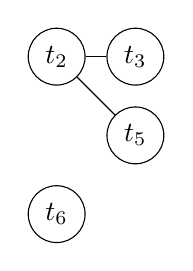
\begin{tikzpicture}
        \graph[nodes={circle, draw}] {
            "$t_2$" -- {"$t_3$", "$t_5$"};
            "$t_6$";
        };
    \end{tikzpicture}
 \end{figure}
 We can then choose the independent sets $t_3, t_5, t_6$ and $t_2$, assigning $3$ codes overall. In this case, eliminating the well-connected vertex $t_4$ also eliminated a clique within the graph, reducing the number of codes which would need to be assigned later, despite $t_4$ not being in the initial maximum independent set.

\section{}
\subsection*{a.}



\begin{thm}
    \label{thm:soln-map}
    Let $n$ be the size of $A$, $K$ be the algorithm for $K1$, $SH: (\mathbb{R} \times \mathbb{R})^n -> (\mathbb{R} \times \mathbb{R})^n$ be a function which circular-shifts a list of point so that the point with minimum x-coordinate is first, and $S(A)$ be $A$ after sorting. Then $S(A) = P^{-1}(SH(K(P(a))))$, that is, 
    if sorting $A$ yields $S(A)$, and applying the algorithm for $K1$ to $P(A)$ yields $C(A)$, then $S(A) = \text{the x-coordinates of } C(A)$. (equivalent up to a circular shift).
\end{thm}
\begin{proof}
    Sorting $A$ yields $S(A)$, which contains exactly the elements of $A$, in order such that, for every $a_j \in S(A) \ s.t. \  j \notin \{1, n\}$, $a_{j-1} \leq a_j$ and $a_{j+1} \geq a_j$ (by the definition of sorting and the transitivity of comparison). We will show that $C(A)$ contains exactly the elements of $P(A)$, and that they are in order such that, for every $(a_j, a_j^2) \in C(A)$, $a_{j-1} \leq a_j$, and $a_{j+1} \geq a_j$ for all $a_j$ except the minimum and maximum values.

    \textbf{Claim: } $\forall a \in \mathbb{R}^2, a \in C(A) \iff a \in P(A)$.
    Suppose $a \notin P(A)$. Since $C(A)$ is by definition a subset of $P(A)$, $a \notin C(A)$. 

    Suppose $a \in P(a)$. Then $a$ lies on the unit parabola. Suppose $a \notin C(A)$. Since $C(A)$ is defined as the convex hull of $P(A)$, this would only happen if there exists a line segment containing $a$ between points within the region bounded by $C(A)$. Since $P(A)$ consists of points on the unit parabola which is convex, the region bounded by $C(A)$ must necessarily exist entirely above the parabola, as otherwise $C(A)$ would either contain points not in $P(A)$, or cease to be convex. If such a line segment existed, it would necessarily intersect with the unit parabola, as otherwise it would not go through $a$. Thus there would be some part of the convex hull of $C(A)$ which exists below the parabola. This contradicts the assumption that $C(A)$ has the same convex hull as $P(A)$, so such a line segment must not exist, and so $a$ must be in $C(A)$. 

    \textbf{Claim: } For all $(a_j, a_j^2) \in C(A)$ other than the first and last, $a_{j-1} \leq a_j$ and $a_{j+1} \geq a_j$. (The x-coordinates are sorted)

    Suppose, without loss of generality, that the algorithm for K1 always starts with the point on $C(A)$ with minimum $x$ value, that is, furthest to the left on the x-y plane. (No matter where the algorithm starts, $C(A)$ can be circular-shifted so that the furthest-left point is first). As all points in $C(A)$ lie on the unit parabola, the next point clockwise from this minimum point must have maximum $x$-coordinate, as otherwise, either the points of $C(A)$ would not lie on the unit parabola, or the area bounded by $C(A)$ would not be convex.

    Then, for a point on $C(A), (a_j, a_j^2)$, $(a_{j-1}, a_{j-1}^2$ is the point on $C(A)$ immediately to the clockwise side of $(a_j, a_j^2)$. Since all $C(A)$ lie on the unit parabola, which is convex upwards, clockwise in this sense indicates that the point has lesser $x$-coordinate (as we have assumed that $a_j$ is not the furthest-left element of $C(A)$). Thus $a_{j-1} \leq a_j$. Similarly, $(a_{j+1}, a_{j+1}^2)$ is the next point in the counterclockwise direction, which in this case, is a point with greater $x$-coordinate, (as we have assumed that $a_j$ is not the furthest-right point of $C(A)$). Thus $a_{j+1} \geq a_j$.

    Therefore, after applying the algorithm for $K1$ to $P(A)$ and applying a circular shift, the $x$-coordinates of the resulting list will contain exactly the elements of $A$ in order, which is the same as the sorted list $S(A)$. Therefore $L1$ reduces to $K1$.
\end{proof}

\pagebreak
Consider the following algorithm: 
\begin{enumerate}
    \item map A to P(A) via the function $x \to (x, x^2)$
    \item Apply the algorithm for K1 to yield the convex hull $C(A)$
    \item Circular-shift the elements of $C(A)$ so that the point with minimum x-coordinate is first 
    \item Map C(A) back to A via the function $(x, x^2) \to x$
\end{enumerate}

By Theorem \ref{thm:soln-map}, this algorithm will produce $A$ sorted. 

Mapping $A$ to $P(A)$ and $C(A)$ to $S(A)$ takes linear time, as an operation is done to each element of $A$. Finding the shift point can also be done in linear time, by iterating through the list. It can also be done in 
$\log(n)$ time with binary search. Since inputs and outputs from $L1$ to $K1$ map in linear time, and a solution to $K1$ yields a solution to $L1$, $L1$ reduces to $K1$ in linear time.

\subsection*{b.}

Let $[]_T$ be the ternary relation on $\mathbb{R}$ defined as $[a, b, c]_T \iff a + b + c = 0$.
Let $[]_{C}$ be the ternary relation on $\mathbb{R}^2$ defined as $[p_1, p_2, p_3] \iff p_1, p_2, p_3 \text{ are collinear}$.

\begin{lem}
    \label{thm:col-eq-zero}
    For $a, b, c \in \mathbb{R}, [a, b, c]_T \iff [(a, a^3), (b, b^3), (c, c^3)]_{C}$.
\end{lem}

\begin{proof}
    Consider the line containing $(a, a^3)$ and $(c, c^3)$. This can be expressed as the equation $y = a^3 + k(x - a)$, where $k = \frac{c^3 - a^3}{c - a}$, equivalently, $y = a^3 + \frac{xc^3 - xa^3 - ac^3 + a^4}{c - a}$. 

    $(b, b^3)$ is collinear with the other two points iff it lies on this line, that is, \begin{align*}
        b^3 &= a^3 + \frac{bc^3 - ba^3 - ac^3 + a^4}{c - a} \\ 
        &= a^3 + (b - a)(c^2 + ca + a^2) \\ 
        &= a^3 + (b-a)((c+a)^2 - ac) \\ 
        &= a^3 + b(c+a)^2 - abc - a(c+a)^2 + a^2c \\ 
        &= a^3 + bc^2 + 2bca + ba^2 - abc - ac^2 - 2a^2c - a^3 + a^2c \\ 
        &= bc^2 + 2bca + ba^2 - abc - ac^2 - 2a^2c + a^2c \\ 
        \\
        0 &= bc^2 + 2bca + ba^2 - abc - ac^2 - 2a^2c + a^2c - b^3 \\ 
        &= bc(c + a) + ba^2 - ac^2 - 2a^2c + a^2c - b^3 \\ 
        &= c(b(c + a) - ac - a^2) + ba^2 - b^3 \\  
        &= c(bc + ab - ac - a^2) + ba^2 - b^3 \\  
        &= c(a+c)(b - a) + ba^2 - b^3 \\  
        &= c(a + c)(b - a) + b(a^2 - b^2) \\  
        &= c(a+c)(b-a) + b(a+b)(a-b) \\  
    \end{align*}

    Suppose $a+b+c = 0$, so $a+b = -c$ and $a+c = -b$.
    Then \begin{align*}
        0 &= c(-b)(b-a) + b(-c)(a-b) \\ 
        &= -bc(b-a) -bc(a-b) \\ 
        &= -bcb + abc - abc + bcb \\ 
        &= 0
    \end{align*}
    Therefore if $a+b+c = 0$, $(a, a^3), (b, b^3)$ and $(c, c^3)$ are collinear. 

    Suppose $a+b+c \neq 0$. Then $a+b+c = k$, where $k \neq 0$, so $a+b = k - c$ and $a + c = k - b$. Then \begin{align*}
        0 &= c(k-b)(b-a) + b(k-c)(a-b) \\ 
        &= c(kb - ka - b^2 + ba) + b(ka - kb - ca + bc) \\ 
        &= ckb - cka - cb^2 + cba + bka - kb^2 - abc + cb^2 \\ 
        &= ckb - cka + bka - kb^2  \\ 
        &= k(cb - ca + ba - b^2) \\ 
        &= k(c(b - a) + b(a - b)) \\ 
    \end{align*}
    Since $k \neq 0$, $k(c(b - a) + b(a-b)) = 0 \iff (c(b-a) + b(a-b)) = 0$. This can only happen if $c = b = 0$, $b-a = a-b = 0$, or $c(b-a) = -b(a-b)$. We will show that under our assumption that $a, b,$ and $c$ are distinct, none of these cases are possible. 

    Consider $c = b = 0$. This contradicts our assumption of distinct values. 

    Consider $b - a = a-b = 0$. This implies $a = -a$ and $b = -b$, so $a = b = 0$, again contradicting our assumption of distinct values. 

    Consider $c(b-a) = -b(a-b)$. Then, \begin{gather*}
        \frac{c}{-b} = \frac{a-b}{b-a} \\ 
        \frac{c}{-b} = \frac{a-b}{-(a-b)} = -1 \\ 
        c = b
    \end{gather*}
    This contradicts our assumption of distinct values. 

    Therefore, $(c(b-a) + b(a-b)) \neq 0$, so $k(c(b-a) + b(a-b)) \neq 0$. Therefore our collinearity equation $0 = k(c(b-a) + b(a-b))$ does not hold. So the the point must not be collinear.

    Therefore, if $a+b+c \neq 0$, $(a, a^3), (b, b^3)$, and $(c, c^3)$ are not collinear.
\end{proof}

\begin{thm}
    \label{thm:iso}
    The structure $\langle \mathbb{R}, []_T \rangle$ is isomorphic to $\langle \chi , []_{C} \rangle$ by $P$, where $\chi = \{(a, a^3) | a \in \mathbb{R}\}$, and $P: \mathbb{R} \to \chi = x \to (x, x^3)$
\end{thm}

\begin{proof}
    Let $P(a) \in \chi = (a, a^3)$. Then $a \in \mathbb{R} = a$. 

    Let $x, y \in \mathbb{R} \  s.t. \  x \neq y$. 

    Then $P(x) = (x, x^2) \neq P(y) = (y, y^2)$. 

    Therefore $P$ is a bijection.

    Let $x, y, z \in \mathbb{R}$. By Lemma \ref{thm:col-eq-zero}, $[x, y, z]_T \iff [(x, x^3), (y, y^3), (z, z^3)]_C$, 
    
    so $[x, y, z]_T \iff [P(x), P(y), P(z)]_C$.

    Since $P$ is bijective and preserves the relation, $P$ is an isomorphism between $\langle \mathbb{R}, T \rangle$ and $\langle \chi, K2 \rangle$.
\end{proof}


Consider the following algorithm which takes the set of points $A$ and returns the set of triplets of points which sum to zero $T(A)$, where $K2$ is the algorithm which finds triplets of collinear points (points which satisfy $[]_T$:
\begin{enumerate}
    \item Map $A$ to $P(A)$ via $a \to (a, a^3)$
    \item Apply the algorithm for K2 to obtain the triplets of points which are collinear, $K2(P(A))$
    \item Map $K2(P(A))$ to $T(A) = P^{-1}(K2(P(A)))$ via $((a, a^3), (b, b^3), (c, c^3)) \to (a, b, c)$
\end{enumerate}

The validity of the final step follows from Theorem \ref{thm:iso}, as the set of triplets which sum to zero exactly corresponds to the set of triplets of points which are collinear (due to the isomorphism). Therefore this algorithm performs the task $L2$ using the algorithm for $K2$, and is thus a reduction of $L2$ to $K2$.

The first mapping visits each element of $A$ once, so it is linear. The second mapping will visit each member of $T(A)$ exactly once, where the upper bound of $T(A)$ is the number of triplets of values in $A$, which is $\binom{|A|}{3} = \frac{|A|!}{(3!)(|A| - k)!} = \frac{|A|(|A| - 1)(|A| - 2)}{3!} \leq |A|^3$, so it is also linear. Therefore $L2$ reduces to $K2$ in linear time.



\end{document}
